\chapter{Android}
	
	%TODO verificar o que esse middleware faz
	Android é um projeto ~\textit{open source} iniciado pela Google, voltado para plataformas de
	dispositivos móveis desenvolvido na linguagem Java, incluindo sistema operacional,
	~\textit{middleware} e aplicações chaves. Inicialmente os celulares não possuíam muita memória,
	isso fazia com que as aplicações Java consumissem boa parte dessa memória. Para contornar esse
	problema, foi desenvolvido uma nova ~\textit{Virtual Machine (VM)} específica denominado de
	~\textit{Dalvik Virtual Machine (DVM)} ~\cite{android}.
	
	Colocar um comentário melhor:
	
	\begin{itemize}
	  \item {~\textit{Dalvik Virtual Machine \\}}
	  
			O ~\textit{DVM} possui um comportamento um pouco diferente quando comparado a ~\textit{JVM}.
			Enquanto que na ~\textit{JVM} a compilação de classes classe gera um arquivo .class específico
			para cada classe, no ~\textit{DVM} a compilação das classes gera um arquivo de extensão
			~\textit{dex} contendo várias classes. O arquivo gerado é otimizado para o melhor uso da memória e
			operações de entrada e saída. \\
	  
	  \item  {~\textit{Software Development Kit} \\}
		
		O Android possui um ~\textit{Software Development Kit (SDK)} próprio. Neste ~\textit{SDK} são
		disponibilizados os recursos necessários para o desenvolvimento das aplicações no ambiente Android
		e trás a possibilidade de emulação de diversos dispositivos para testes dessas aplicações. \\
		
	  \item {~\textit{Native Development Kit} \\}		
	
		A plataforma do Android aceita aplicações que sejam desenvolvidas com a linguagem Java. No entanto,
		é possível combinar aplicações Java com aplicações e bibliotecas desenvolvidas em C/C++ utilizando
		a ~\textit{Java Native Interface (JNI)} através do ~\textit{Native Development Kit (NDK)}. \\
	
	\end{itemize}

	\section{Arquitetura}
	
		A figura ~\ref{androidArquitetura} apresenta como a arquitetura do Android está dividida em camadas.
		Sendo estas divididas em:
	
		\begin{itemize}
			\item{ ~\emph{Aplications} \\}
			
				Nesta camada ficam as aplicações propriamente ditas, as quais são manipuladas pelo usuário
				final. Sendo composta por funções básicas do dispositivo, como por exemplo, realizar chamada,
				navegar na internet, acessar lista de contatos, dentre outras. \\
			
			\item{~\emph{Aplication Framework} \\}
			
				Descendo para a próxima camada temos a camada responsável pelas funções de gerenciamento do
				telefone. Nesta camada é possível encontrar um conjunto de componentes voltados para o auxílio
				no desenvolvimento de aplicações, disponibilizadas em ~\textit{Application Programming Interface
				(API)} e recursos necessários para os pacotes e aplicativos, tais como classes visuais (botões
				e ~\textit{views}), troca de recursos entre aplicativos, gerenciamento dos recursos, ciclo de
				vida de aplicações e gerenciamento de pacotes. \\
					
			\item{~\emph{Libraries} \\}
			
				Aqui são incluídas as bibliotecas do Android, muitas delas desenvolvidas em C/C++ e são
				utilizadas por diversos componentes do sistema. Estas bibliotecas possuem conjuntos de
				instruções que facilitam o desenvolvimento de aplicações, dando suporte a camada superior.
				O conjunto de bibliotecas extende-se desde a manipulação de arquivos de mídia, imagem e vídeo,
				oferecendo suporte a exibição de conteúdos bidimensionais e tri diomensionais, baseados no
				OpenGL, chegando até a manipulação de dados em banco de dados com o SQLite.\\
				
			\item{~\emph{Android Runtime} \\}
			
				É nesta camada que o ~\textit{DVM} reside e divide espaço com as bibliotecas principais do
				sistema. Essas bibliotecas fornecem a maioria das funcionalidades disponíveis. Um ponto interessante
				implementado nessa arquitetura é a utilização de instâncias ~\textit{DVM} para cada processo, ou
				seja, cada aplicação possui seu próprio processo e sua própria instância da ~\textit{DVM}. \\

			\item{~\emph{Linux Kernel} \\}
			
				Essa camada atua como uma camada de abstração entre o hardware e o software. Fica responsável
				pelo gerenciamento de memória e processos, rede e ~\textit{drivers} de conexão. \\
				
		\end{itemize}
	
	
		\begin{figure}[h]
			\centering 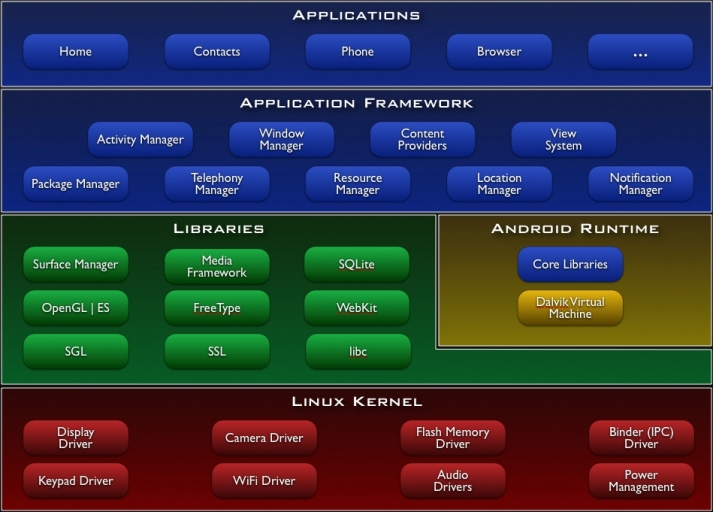
\includegraphics[scale=.65]{figuras/anexos/androidArquitetura.jpg}
			\caption{\textit{Arquitetura do Android ~\cite{android}.}}
			\label{androidArquitetura} 
		\end{figure}
	

